\section{Integration and Test Facility (ITF)}
\label{sec:fdsp-tc-itf}

%%%%%%%%%%%%%%%%%%%%%%%%%%%%
\subsection{Introduction}
\label{sec:fdsp-tc-itf-intro}

The components of the DUNE detectors will be manufactured in many numerous different countries and locations. 
For many of the parts it is reasonable to ship the components to the logistics warehouse and then receive the equipment underground where it can be installed. 
However the  cold electronics and the photon detectors are tightly coupled to the APA. 
The wires and filters on the APA form part of the electronics circuit and the photon supports and cabling are built into the APA. 
The work to integrate the CE and PD into the APA is large and the risk of damaging the components is significant, so it is planned to integrate the components as early as possible and then thoroughly test the complete assembly.
In order to avoid having to create integration testing facilities at each factory one central facility will be established in South Dakota near the SURF site  (within 1 hour drive). 
In this Integration Test Facility (ITF) the APA, CE and PD modules will arrive, undergo initial tests, be integrated together, undergo a set of warm tests. 

As the CE electronics will be available roughly 2 years before the start of installation the ITF needs to be available on the same time scale. Other components are available earlier. 
The specifications for the ITF are summarized in Table \ref{tab:specs:just:SP-TC}.  
The ITF relevant specifications are the quality of the cleanroom and the specification on the UV filtering of the light for the photon detectors.



%\begin{dunetable}
%[ITF Specifications]
%{cc}
%{tab:tcps-itf-spec}
%{Summary of the high level specifications for the ITF. %The building requirements are covered separately in a separate section.}
%Parameter & Specification \\ \toprowrule
%Cleanroom & The ITF cleanroom shall meet ISO-8 standard per ISO-14644 \\ \colhline
%Filtered Lights & <520 nm for long exposure and <400 %for exposures less than 2 weeks \\ 
%\end{dunetable}



%%%%%%%%%%%%%%%%%%%%%%%%%%%%
\subsection{APA-CE-PD integration}
\label{sec:fdsp-tc-itf-integ}

\begin{dunefigure}[ITF cleanroom layout]{fig:fdsp-tc-itf-clean}
{Conceptual layout of the cleanroom for the APA-CE-PD integration and testing.}
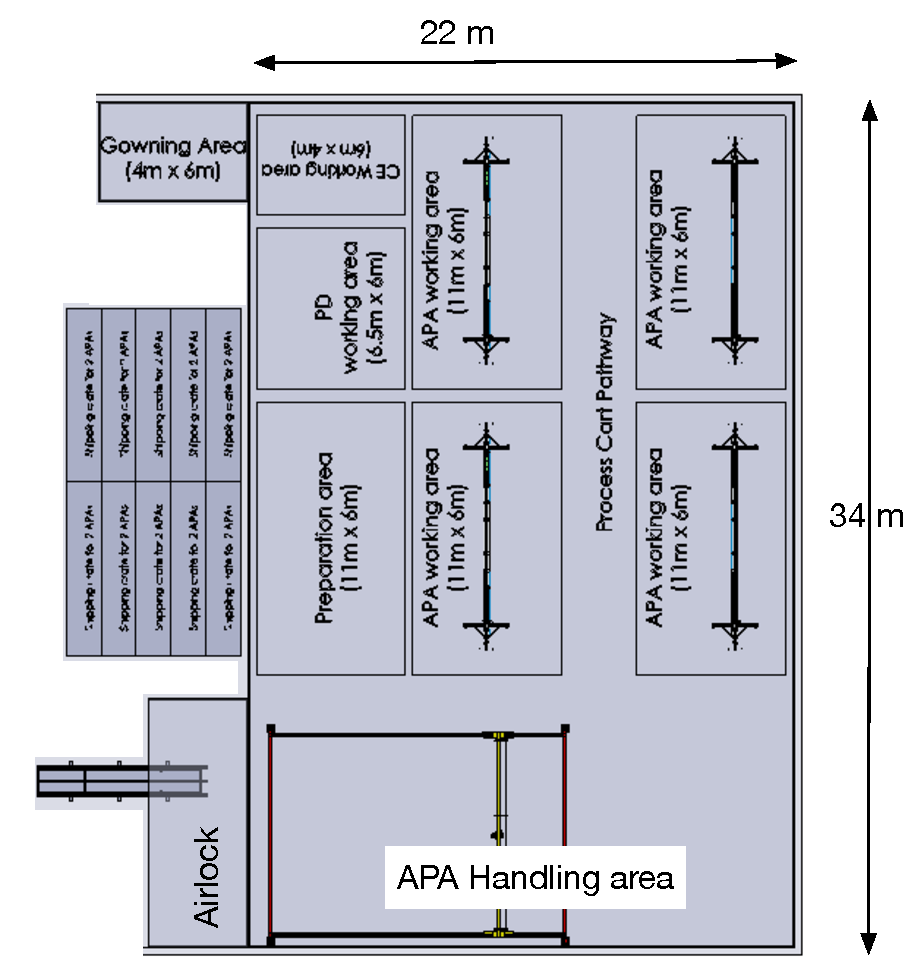
\includegraphics[width=0.8\textwidth]{itf-cleanroom-v2}
\end{dunefigure}

Most the work in the ITF must be done in a cleanroom environment to protect the components from dust and unfiltered light. The cleanliness requirement for the detector components is ISO-8 which corresponds to filtered air with clean lab coats, clean shoes, and hair nets. 
To protect the photon detector's \dword{wls} coating the lights need to be filtered to remove frequencies below 520nm.\cite{LBNE-docdb-8348} One possible layout of the cleanroom is shown in Figure \ref{fig:fdsp-tc-itf-clean}.
Materials enter the ITF cleanroom through the materials airlock. This area needs to be sufficiently large to accommodate the APA transport boxes and allow workers to move around the box to remove the dirty shipping layer and prepare for transport into the cleanroom. 
Other materials will also be brought into the cleanroom through the airlock, but they will need much less space than the APA crates. Figure \ref{fig:fdsp-tc-itf-clean} shows an APA transport box being moved into the airlock on the lower right.
The CE and PD equipment will be moved to the PD and CE work areas respectively. 
Here the components are unpacked and tested prior to integration in the APA. 
The tests performed are described in more detail in the QA/QC section below. 

The APA enter cleanroom through the airlock and initially go to the APA handling area where an overhead workstation or gantry crane will be available. 
The APA will then be removed from the transport box and mounted to a process cart which can rotate the APA horizontally. The process cart will be pushed to one of the four APA integration areas and then prepared for the installation of the CE and PD. 
During the integration process the APA will be held horizontal and the PDs will be inserted into the sides while the cold electronic boxes are mounted to the end of the APA. 
After the component integration the system will be tested and then either moved back to the handling area and boxed for return to the logistics center for storage.  

All the detector  components will arrive at the ITF either from the logistics facility or directly from the factories. Sufficient space will be needed inside the ITF but outside the cleanroom to store several weeks of material and a few boxes of the integrated APA boxes. Additionally a changing room is needed for the workers to change into clean cloths and shoes. The capacity of the changing room should be sufficient for roughly 10-20 workers in the cleanroom. 

%%%%%%%%%%%%%%%%%%%%%%%%%%%%
\subsection{ITF QA/QC}
\label{sec:fdsp-tc-itf-qaqc}
Extensive testing of the detector components will be performed inside the IFT facility as the APA-PD-CE integration takes place. These tests form a vital part of the quality control process for DUNE. Details of the tests for each of the components are described below.

\subsubsection{APA}
The APA will be unpacked from the transport box, installed on the process cart and the protective shields removed to allow a detailed visual inspection. Then it will be transported to the integration area, where it will be held horizontally. The main test to be performed at this stage, i.e. before the integration with the photon detectors and the cold electronics, is tension measurement. Ideally, all wires would be measured to ensure that they were no changes during the shipping. The limiting factor of the tension measurement will be time. In the current plan, about 350 wires, representing 10$\%$ of the total, will be measured, which will take 3 shifts with 2 people. All the measured values will be stored in the wire QC database. In the current plan, the tension measurement will be performed using the laser method, the same method used at the Production Site. This method utilizes a laser focused on individual wires to be measured. By plucking the wire to induce a vibration, a photodiode under the wire records the frequency of vibration, which directly translates into tension value. While this method is robust and has been extensively used by LArTPC experiments, it is very time consuming. An alternative method, using electrical signals is currently under development and could replace the laser method, potentially allowing to measure all the APA wires at the ITF in the same amount of time or less.

The current requirement for the tension values are 6$\pm$1 N and wires measured to be outside this range will be removed from the APA. Note that the exact tolerance is currently under study with protoDUNE data to ensure the required acceptable range that could lead to the removal of a channel otherwise.

The last test to be performed to ensure the quality of an APA is the wire continuity. This checks that all the wires are still intact and still well connected to the readout boards. This test can easily be done once the cold electronics is installed (see next sub-section).    
\subsubsection{Cold Electronics}
The QA for the CE is described in the CE chapter.

\subsubsection{Photon Detectors}

Photon detectors will arrive at the \dword{itf} in custom designed crates.  Each crate will contain the ten photon detector modules required for a single APA.  
Each photon detector comes individually packaged in a static-resistant sealed plastic bag, filled with clean dry nitrogen.

Prior to integration into an APA, each PD module is removed from it's shipping bag and undergoes a visual inspection. 
Modules passing initial inspection are then loaded into the optical scanner for operational testing.

The \dword{pd} optical scanner allows testing of the operation of the photosensor readout chain to ensure all the electrical connections are operational, while also measuring the light-collection performance at several positions along the length of the module.  
Duplicate identical optical scanners are used at the module assembly facility, where a scan represents the last \dword{qc} test prior to shipping to the \dword{itf} and again immediately prior to installation, allowing for a sensitive test for changes in module performance due to shipping or storage.  
This technique was used successfully in \dword{pdsp}, and will be replicated for \dword{dune}

The optical scanner consists of a light-tight box, approximately \num{2.5}m long, with a \num{0.75} $\times$ \num{0.75}m cross section. 
The box is fabricated from aluminum, and acts as a Faraday cage to minimize electrical interference with measurements. 
In the \dword{dune} configuration, two PD modules to be tested are inserted into the station through slots face of the box, guided by support rails of the type used in the APAs, representing a final mechanical check of the dimensions of the module.  
Electrical connection to the module is made using an electrical connector identical to that in the APA frames, allowing for a final check of that crucial interface.
Following insertion in the scanner, the the insertion slots are closed and optically sealed, and the scan begins. 
\dword{dune} \dword{pd} readout electronics are used to bias and read out the module photosensors, while a UV LED is scanned along the length of the modules by an automated stepper-motor driven translation stage.  
Measurements of detector response are made at 16 positions along the length of the module, (on two sides in the case of double-sided \dword{pd} modules), checking the performance of each of the dichroic filters. 
The response is compared to that measured in the assembly facility. 
Figure \ref{fig:fdsp-tc-pds-scanner} shows the scanner used to test the \dword{pdsp} photon detectors.


\begin{dunefigure}[Photon detector scanner]{fig:fdsp-tc-pds-scanner}
{Picture of the scanner for operational tests of the \dword{pd} modules before integration into the APAs.}
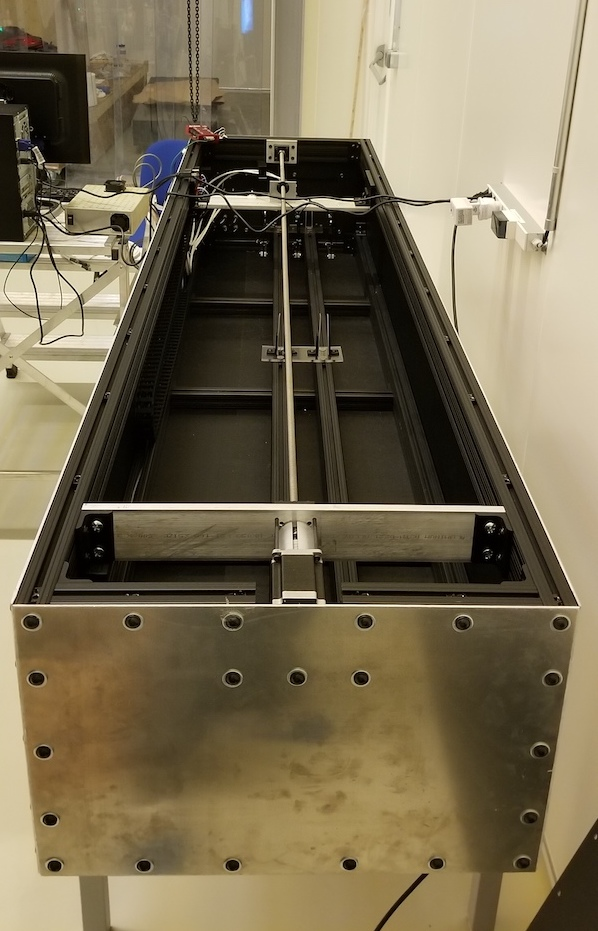
\includegraphics[height=.60\textheight, angle=0]{pds-scanner}
%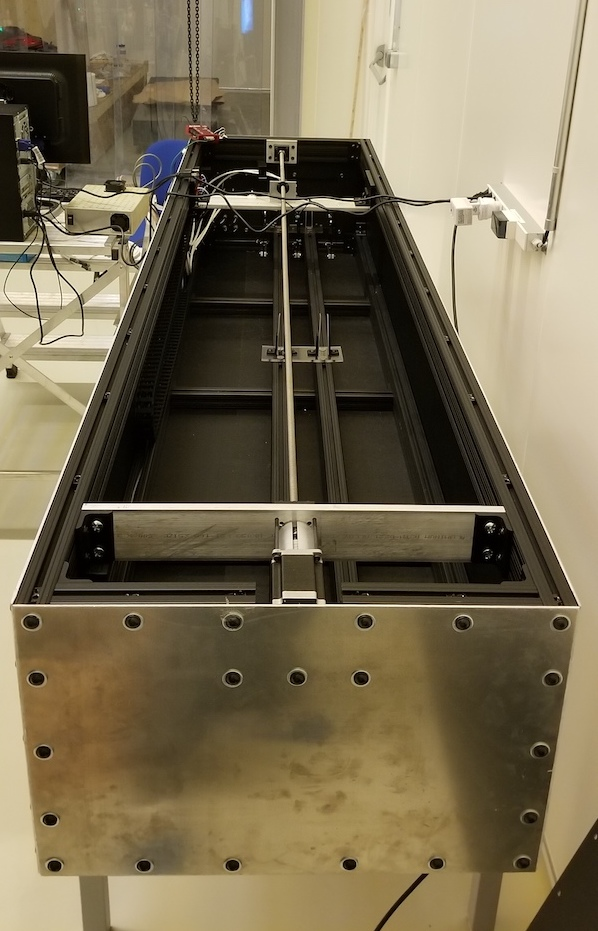
\includegraphics[width=1.0\textwidth, angle=-90]{pds-scanner}
\end{dunefigure}

Photon detector insertion into the \dwords{apa} immediately follows optical scanning.  
Modules are inserted into the \dword{pd} support rails, where the connection to the cable harness pre-installed in the \dword{apa} prior to wire wrapping is automatically made as part of insertion.  
Immediately upon insertion, an electrical continuity check is made, checking the continuity between the PD module and the \dword{pd} cable end connector where it exits the end of the \dword{apa}



%%%%%%%%%%%%%%%%%%%%%%%%%%%%
\subsection{Building Requirements and Infrastructure}
\label{sec:fdsp-tc-itf-req}
The ITF building requirements are summarized in DocDb 11500.\cite{bib:docdb11500} The building to be used as the ITF facility has not been identified at present. In order to assist in identify or designing the ITF building a set of requirements were drafted. The requirements document defines the spaces needed for the integration work while not specifying the final layout of the cleanroom. This will allow the configuration of the cleanroom spaces to be adapted to possible building footprints as candidate buildings are identified. As the building has not been identified the cleanroom layout shown in Figure \ref{fig:fdsp-tc-itf-clean} should be taken as a concept and the final layout may change to adapt to the footprint of the final building. The building requirements document\cite{docdb-11500}  defines the minimum spaces for all the operations inside the ITF cleanroom, it defines the space needed for the cold box and the related cryogenic system, it provides guidance for the space needed for material storage outside the cleanroom, and it established the power and other general requirements the building must fulfill. Some requirements depend on the location of the building and the facilities available in the area. For example office space for 20 scientists working in the ITF will be needed in the area, but this would not need to be in the ITF building if local options are available. Some local machining facilities also fall into this category. 

%%%%%%%%%%%%%%%%%%%%%%%%%%%%
\subsection{Safety}
\label{sec:fdsp-tc-itf-safety}

Integration and Testing Facility safety is identical to the information listed in section 1.1.4 Logistics Safety as it is also operated by SDSD as a Fermilab Facility.    If the ITF and Logistics facility are located near each other a safety officer can be shared by the two sites.    

%%%%%%%%%%%%%%%%%%%%%%%%%%%%
\subsection{Cost, Schedule and Risk Analysis}
\label{sec:fdsp-tc-itf-cost}

\fixme{Add costs when they are available}

{\bf ITF Time line and APA Integration Schedule}
The time line for the start-up for ITF operational in 2022 when there are Photon Detectors and Cold Electronics are available to integrate.  This gives two years for integrate APAs before installation begins. The pros of this schedule is the ability to test all the integrated components as soon as possible minimizing and schedule risk if there are problems. Smaller integration team size would be required since the time-scale is stretched reducing labor costs. Since the schedule for integrating the components is less it is feasible to start closer to one year before detector installation. 

Using 4 work stations and working only day shift it takes approximately 9 shifts to complete an APA pair as shown in figure \ref{fig:ITF-Schedule}

\begin{dunefigure}[Schedule APA Integration in ITF]
{fig:ITF-Schedule}
    {ITF-Schedule}
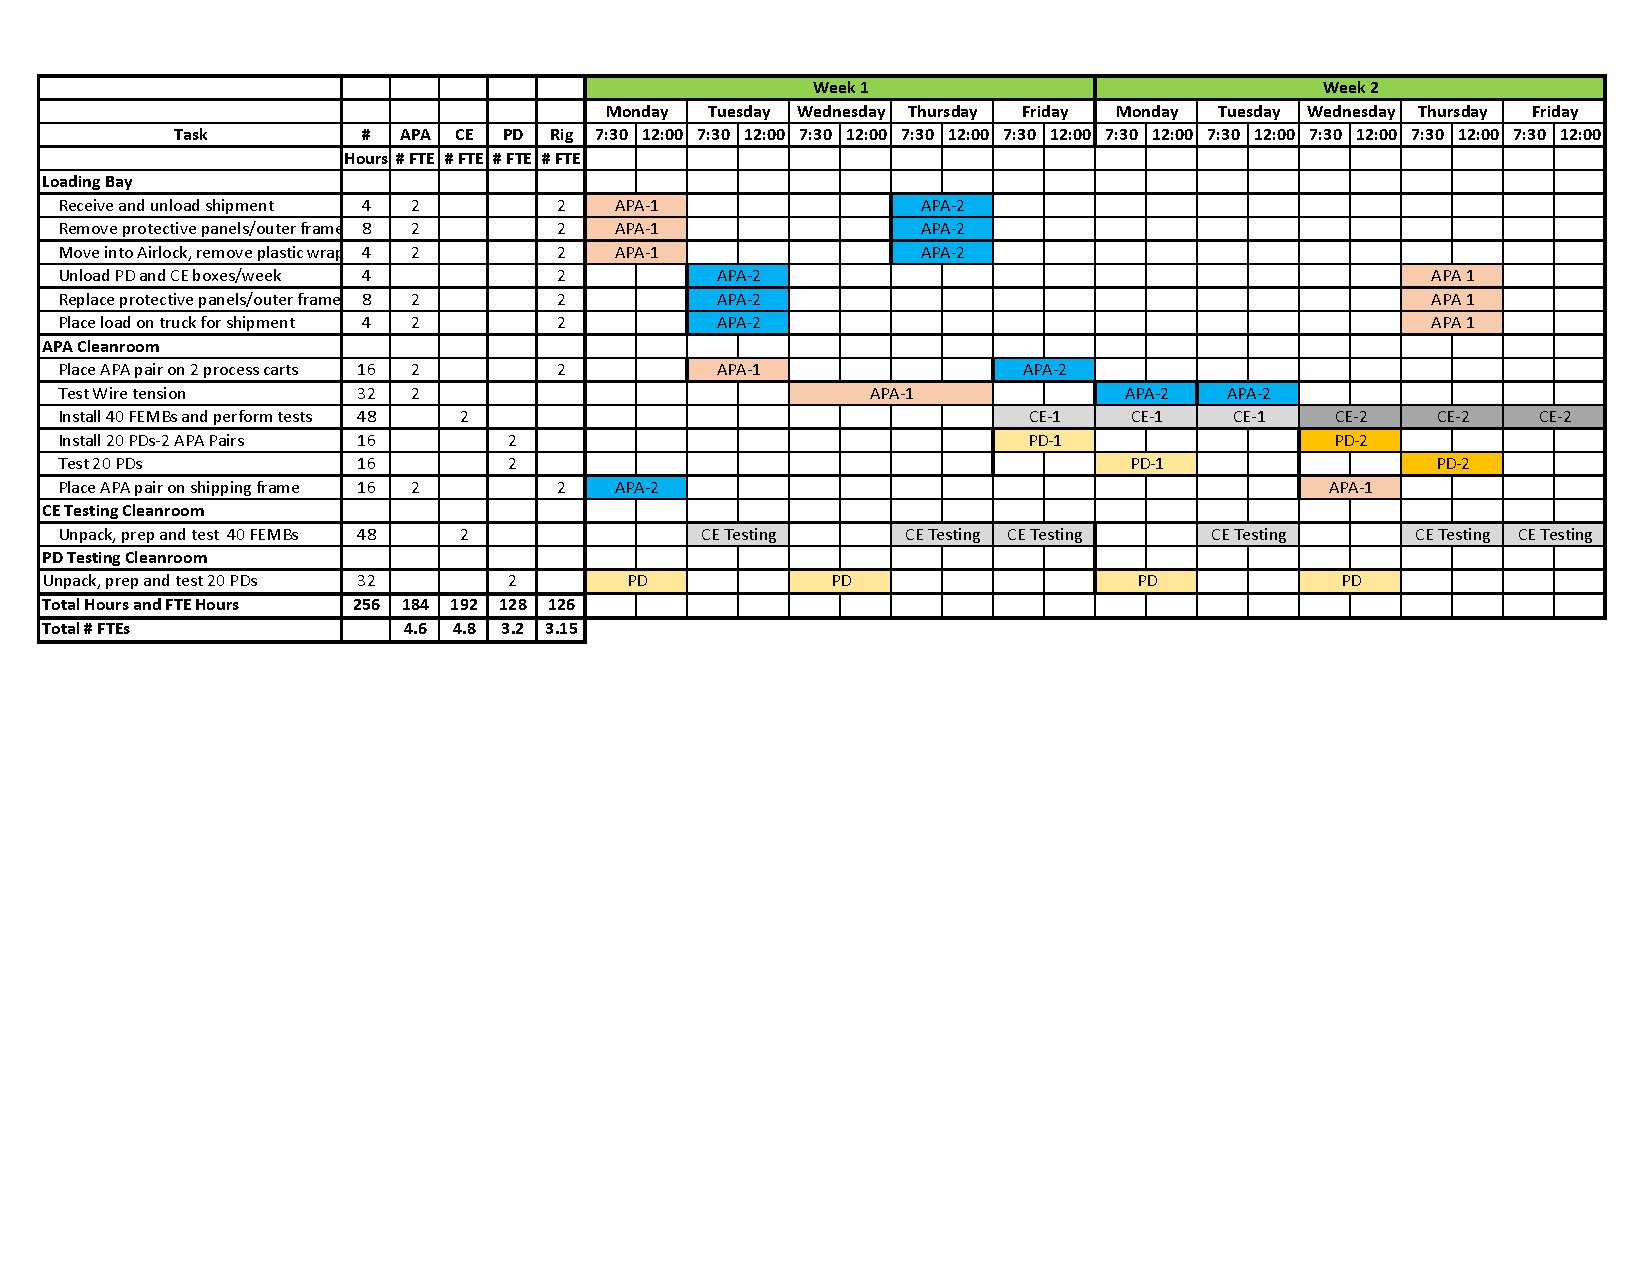
\includegraphics[width=0.98\textwidth]
{ITF-Schedule} 
\end{dunefigure}


\fixme{use templates from cost-risk-sched.tex file. Anne}
